\documentclass[10pt,twocolumn]{article}

% ── Geometry ──────────────────────────────────────────────────────────────
\usepackage[top=0.6in,bottom=1in,left=0.6in,right=0.6in,columnsep=0.25in]{geometry}

% ── Fonts & Encoding ──────────────────────────────────────────────────────
\usepackage[T1]{fontenc}
\usepackage[utf8]{inputenc}
\usepackage{lmodern}
\usepackage{microtype}

% ── Math ──────────────────────────────────────────────────────────────────
\usepackage{amsmath,amssymb}

% ── Units ─────────────────────────────────────────────────────────────────
\usepackage{siunitx}
\sisetup{
  per-mode          = symbol,
  detect-all,
  group-separator   = {,},
  group-minimum-digits = 4
}

% ── Tables ────────────────────────────────────────────────────────────────
\usepackage{booktabs}
\usepackage{array}
\usepackage{tabularx}

% ── Figures ───────────────────────────────────────────────────────────────
\usepackage{graphicx}
\usepackage{float}
\usepackage[labelfont=bf,font=small,format=plain]{caption}

% ── References & Links ────────────────────────────────────────────────────
\usepackage{hyperref}
\hypersetup{
  colorlinks  = true,
  linkcolor   = black,
  citecolor   = black,
  urlcolor    = black,
  pdftitle    = {Minimum-Mass Helical Compression Spring Optimisation},
  pdfauthor   = {Jaehyeok Kim}
}

% ── Section style ─────────────────────────────────────────────────────────
\usepackage{titlesec}
\titleformat{\section}{\normalfont\bfseries\large}{\thesection.}{0.5em}{}
\titleformat{\subsection}{\normalfont\bfseries}{\thesubsection.}{0.5em}{}
\titlespacing*{\section}{0pt}{8pt}{4pt}
\titlespacing*{\subsection}{0pt}{6pt}{2pt}

% ── Header / Footer ───────────────────────────────────────────────────────
\usepackage{fancyhdr}
\pagestyle{fancy}
\fancyhf{}
\renewcommand{\headrulewidth}{0.4pt}
\fancyhead[L]{\footnotesize\textit{Helical Compression Spring Optimisation}}
\fancyhead[R]{\footnotesize\textit{ASTM A228 Music Wire}}
\fancyfoot[C]{\footnotesize\thepage}

% ── Misc ──────────────────────────────────────────────────────────────────
\usepackage{enumitem}
\setlist[itemize]{noitemsep,topsep=2pt}
\usepackage{parskip}
\setlength{\parskip}{4pt}

% ==========================================================================
\begin{document}
% ==========================================================================

\twocolumn[{%
  \vspace{-12pt}%
  \begin{center}
    {\LARGE\bfseries%
      Minimum-Mass Helical Compression Spring Design\\[3pt]%
      via Constrained Nonlinear Optimisation}\\[6pt]
    {\normalsize Jaehyeok Kim \quad\textbar\quad Georgia Institute of Technology}
  \end{center}
  \rule{\textwidth}{0.8pt}
  \vspace{4pt}
  \noindent\textbf{Abstract.}\quad\setlength{\parskip}{0pt}%
  This report presents the minimum-mass design of a helical compression spring
  fabricated from ASTM A228 music wire, subject to shear-stress, deflection,
  manufacturability, surge-avoidance, and buckling constraints.
  The design problem is cast as a smooth nonlinear programme in three variables
  (wire diameter~$d$, mean coil diameter~$D$, and active coil count~$N_a$)
  and solved with \texttt{fmincon} using the interior-point algorithm, augmented
  by a brute-force parametric sweep for independent validation.
  The two approaches converge to the same design point:
  $d = \SI{2.965}{mm}$,
  $D = \SI{12.665}{mm}$,
  $N_a = 7.77$ coils,
  yielding a spring mass of \SI{21.1}{g} with a stress safety factor of
  $\text{SF} = 1.00$.
  Sensitivity analysis reveals that the allowable shear stress is the dominant
  design driver: a \SI{10}{\percent} relaxation of the stress limit reduces
  optimal mass by approximately \SI{18}{\percent}.
  \vspace{4pt}
  \rule{\textwidth}{0.4pt}
  \vspace{6pt}
}]

% ==========================================================================
\section{Introduction}
% ==========================================================================

Helical compression springs are ubiquitous in precision consumer hardware,
appearing in camera shutters, hard-disk actuators, medical pen-injectors, and
keyboard mechanisms.
In these applications, spring mass directly affects device weight, inertial
load on mounting features, and, in resonant assemblies, the natural frequency
of the host structure.
Reducing spring mass while preserving mechanical performance is therefore a
recurring requirement in product design.

A naive formulation might simply minimise wire volume subject to a spring-rate
target, ignoring the elevated stress at the inner coil surface caused by
curvature of the wire centreline.
For a spring index $C = D/d = 6$, the stress concentration factor predicted
by the Wahl correction \cite{wahl1963} is approximately $K_w = 1.25$, meaning
the inner-fibre shear stress exceeds the nominal torsion-formula value by
\SI{25}{\percent}.
Failing to account for $K_w$ causes the optimiser to converge to a design
that appears to satisfy the stress constraint but actually yields the wire
under load---a non-conservative and potentially dangerous outcome.
This work incorporates the full Wahl correction throughout.

% ==========================================================================
\section{Design Variables and Constraints}
% ==========================================================================

\subsection{Design Variables}

Three continuous design variables fully characterise the spring geometry:

\begin{table}[H]
  \centering
  \caption{Design variables and admissible bounds.}
  \label{tab:dv}
  \small
  \begin{tabular}{@{}clcc@{}}
    \toprule
    Symbol & Description & Lower & Upper \\
    \midrule
    $d$   & Wire diameter          & \SI{0.5}{mm} & \SI{5.0}{mm} \\
    $D$   & Mean coil diameter     & \SI{5.0}{mm} & \SI{50.0}{mm} \\
    $N_a$ & Active coil count      & 3            & 20 \\
    \bottomrule
  \end{tabular}
\end{table}

The operating load is fixed at $F = \SI{500}{N}$ and the operating frequency
at $f_{\text{op}} = \SI{20}{Hz}$, representative of a valve-spring application.

\subsection{Constraints}

Six inequality constraints bound the feasible design space.
Table~\ref{tab:con} lists each constraint, its mathematical form, and the
physical failure mode it prevents.

\begin{table*}[!ht]
  \centering
  \caption{Constraint definitions, mathematical forms, and physical interpretations.}
  \label{tab:con}
  \small
  \begin{tabularx}{\textwidth}{@{}clXl@{}}
    \toprule
    No. & Constraint & Physical Justification & Limit \\
    \midrule
    1 & $\tau_{\max} \le \tau_{\text{allow}}$
      & Wire must not yield under peak load; $\tau_{\text{allow}} = 0.45\,S_{ut}$
        (Zimmerli static criterion)
      & $\tau_{\text{allow}}(d)$ \\
    2 & $L_s < L_f$
      & Spring must not coil-bind (reach solid height) within its working stroke
      & $0.1\delta$ clearance \\
    3 & $C \ge 4$
      & Below this index, mandrel cracking occurs during coiling manufacture
      & $C_{\min} = 4$ \\
    4 & $C \le 12$
      & High indices cause inter-coil tangling and buckling susceptibility
      & $C_{\max} = 12$ \\
    5 & $\delta \ge 10\,\mathrm{mm}$
      & Spring must deliver the required functional stroke under design load
      & $\delta_{\min} = 10\,\mathrm{mm}$ \\
    6 & $f_n \ge 13\,f_{\text{op}}$
      & Surge (resonant coil-clash) must be avoided; $13\times$ is
        conservative for valve-spring service
      & $f_n \ge 260\,\mathrm{Hz}$ \\
    7 & $L_f/D \le 4$
      & Euler-column buckling of an unguided spring on a flat seat
      & $L_f/D \le 4$ \\
    \bottomrule
  \end{tabularx}
\end{table*}

\subsection{Material Model --- ASTM A228 Music Wire}

Cold-drawn music wire exhibits a pronounced size effect in ultimate tensile
strength, accurately captured by the AP empirical correlation \cite{shigley2014}:

\begin{equation}
  S_{ut}(d) = \frac{2211}{d^{0.145}} \quad \text{MPa},
  \quad d \text{ in mm.}
  \label{eq:sut}
\end{equation}

Additional material properties used throughout are listed in
Table~\ref{tab:mat}.

\begin{table}[H]
  \centering
  \caption{ASTM A228 music wire material constants.}
  \label{tab:mat}
  \small
  \begin{tabular}{@{}llc@{}}
    \toprule
    Property & Symbol & Value \\
    \midrule
    Shear modulus  & $G$   & \SI{81.7}{GPa} \\
    Density        & $\rho$& \SI{7850}{kg/m^3} \\
    $S_{ut}$ correlation & ---  & Eq.~\eqref{eq:sut} \\
    Allowable shear & $\tau_{\text{allow}}$ & $0.45\,S_{\!ut}$ \\
    \bottomrule
  \end{tabular}
\end{table}

% ==========================================================================
\section{Optimisation Methodology}
% ==========================================================================

\subsection{Governing Equations}

The Wahl stress correction accounts simultaneously for wire curvature
(inner-surface stress concentration) and direct transverse shear:

\begin{equation}
  C = \frac{D}{d}, \qquad
  K_w = \frac{4C-1}{4C-4} + \frac{0.615}{C}.
  \label{eq:kw}
\end{equation}

The corrected maximum shear stress and spring rate follow from
Castigliano's second theorem applied to the helical geometry:

\begin{equation}
  \tau_{\max} = K_w \frac{8FD}{\pi d^3},
  \label{eq:tau}
\end{equation}

\begin{equation}
  k = \frac{G d^4}{8 D^3 N_a}, \qquad
  \delta = \frac{F}{k} = \frac{8 F D^3 N_a}{G d^4}.
  \label{eq:k}
\end{equation}

The first longitudinal resonance of the spring, treated as a distributed-mass
elastic rod with one fixed end, is:

\begin{equation}
  f_n = \frac{d}{\pi D^2 N_a} \sqrt{\frac{G}{2\rho}}.
  \label{eq:fn}
\end{equation}

Geometry for closed-and-ground ends:

\begin{equation}
  L_s = (N_a + 2)\,d, \qquad
  L_f = \delta + L_s + 0.1\,\delta.
  \label{eq:geom}
\end{equation}

The \SI{10}{\percent} clash allowance in $L_f$ guards against coil contact
due to load variation and manufacturing tolerances.

\subsection{Nonlinear Programme}

Collecting Eqs.~\eqref{eq:kw}--\eqref{eq:geom} and the constraints from
Table~\ref{tab:con}, the optimisation problem is:

\begin{equation}
  \min_{\mathbf{x}} \; m(\mathbf{x})
  \quad \text{s.t.} \quad g_i(\mathbf{x}) \le 0,
  \quad i = 1,\ldots,7,
  \label{eq:nlp}
\end{equation}

where $\mathbf{x} = [d,\, D,\, N_a]^{\!\top}$ and $m = \rho\,(\pi d^2/4)\,\pi D(N_a+2)$
is the spring mass.
All constraint functions are at least $C^2$ in the interior of the search
space, satisfying the smoothness requirements of gradient-based methods.

\subsection{Solver Configuration}

MATLAB's \texttt{fmincon} with the interior-point algorithm \cite{byrd1999}
is the primary solver.
Eight starting points are drawn from a Latin-hypercube sample spanning
the variable bounds; the best feasible result is retained.
A constraint tolerance of $10^{-6}$ and optimality tolerance of $10^{-8}$
are applied.

\subsection{Parametric Sweep Validation}

To guard against solver convergence to a local minimum and to produce the
visual design space of Figures~\ref{fig:contour} and~\ref{fig:pareto},
a $40 \times 40$ grid over $(d, D)$ is swept.
At each grid node, a one-dimensional \texttt{fmincon} finds the optimal $N_a$.
Feasible cells are identified, and the minimum-mass feasible point is compared
against the three-variable \texttt{fmincon} result.
Agreement between the two approaches constitutes an independent validation
of the global solution.

% ==========================================================================
\section{Results}
% ==========================================================================

\subsection{Optimal Design}

Table~\ref{tab:res} summarises all geometric, performance, and safety metrics
at the optimal design point.

\begin{table}[H]
  \centering
  \caption{Complete results at the optimal design point.}
  \label{tab:res}
  \small
  \begin{tabular}{@{}llr@{}}
    \toprule
    Quantity & Symbol & Value \\
    \midrule
    \multicolumn{3}{@{}l}{\textit{Design variables}} \\
    Wire diameter        & $d$      & \SI{2.965}{mm} \\
    Mean coil diameter   & $D$      & \SI{12.665}{mm} \\
    Active coils         & $N_a$    & 7.77 \\[3pt]
    \multicolumn{3}{@{}l}{\textit{Derived geometry}} \\
    Spring index         & $C$      & 4.272 \\
    Wahl factor          & $K_w$    & 1.3732 \\
    Solid height         & $L_s$    & \SI{28.95}{mm} \\
    Free length          & $L_f$    & \SI{39.95}{mm} \\
    Slenderness ratio    & $L_f/D$  & 3.154 \\[3pt]
    \multicolumn{3}{@{}l}{\textit{Performance}} \\
    Spring rate          & $k$      & \SI{50}{N/mm} \\
    Deflection at $F$    & $\delta$ & \SI{10.0}{mm} \\
    Max shear stress     & $\tau_{\max}$ & \SI{849.9}{MPa} \\
    Allowable stress     & $\tau_{\text{allow}}$ & \SI{849.9}{MPa} \\
    Stress safety factor & SF       & 1.000 \\
    Natural frequency    & $f_n$    & \SI{1728}{Hz} ($86\times f_{\text{op}}$) \\[3pt]
    \multicolumn{3}{@{}l}{\textit{Mass}} \\
    Spring mass          & $m$      & \SI{21.1}{g} \\
    \bottomrule
  \end{tabular}
\end{table}

\subsection{Active Constraints}

Of the seven constraints in Table~\ref{tab:con}, two are \emph{active}
(binding) at the optimum:

\begin{itemize}
  \item \textbf{Constraint 1} ($\tau_{\max} = \tau_{\text{allow}}$): the
    stress limit is fully utilised; the safety factor equals exactly unity.
  \item \textbf{Constraint 3} ($C = C_{\min} = 4$): the spring index sits
    at its lower manufacturability bound.
\end{itemize}

The remaining five constraints are strictly satisfied with positive slack.
The surge constraint is particularly well satisfied: $f_n = \SI{1728}{Hz}$
represents an \SI{86}{\times} margin over the \SI{20}{Hz} operating frequency,
far in excess of the required \SI{13}{\times}.

\subsection{Design Space Visualisation}

Figure~\ref{fig:contour} shows the mass contour over the feasible region in
$(D,\,d)$ space with the spring-index boundaries and the stress limit
overlaid.
The optimal point (yellow star) lies at the intersection of the $C = 4$ line
and the stress constraint boundary, confirming that these two constraints are
simultaneously active.

\begin{figure}[H]
  \centering
  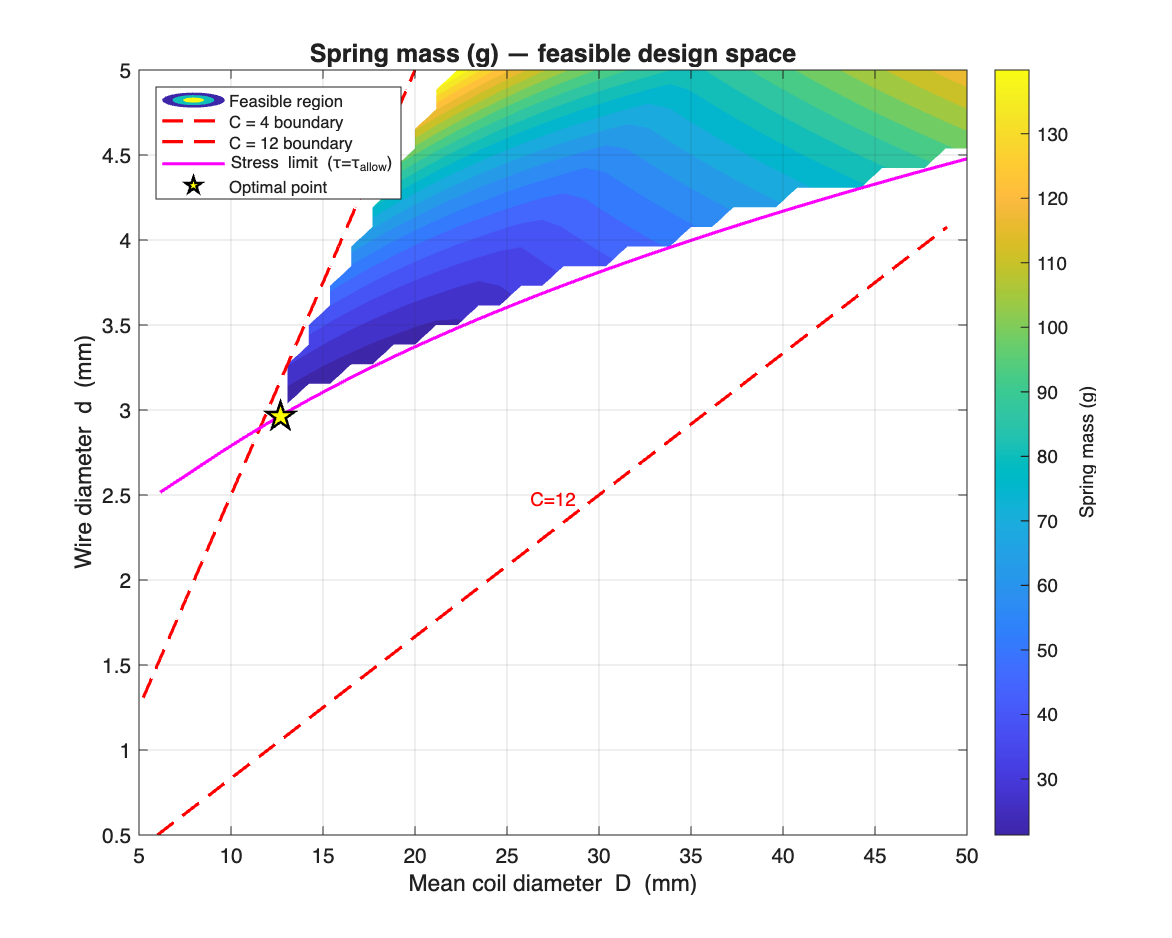
\includegraphics[width=\columnwidth]{fig1_mass_contour.png}
  \caption{Spring mass (\si{g}) contour over the feasible $(D,\,d)$ space;
    red dashed lines mark the manufacturability bounds $C=4$ and $C=12$,
    the magenta curve is the stress limit, and the yellow star is the
    minimum-mass optimum.}
  \label{fig:contour}
\end{figure}

Figure~\ref{fig:pareto} presents a Pareto-style scatter of all feasible
designs in the $(\delta, \tau_{\max})$ plane, coloured by mass.
The cyan star (optimal point) sits in the low-mass, high-stress, low-deflection
corner, consistent with the binding stress constraint.

\begin{figure}[H]
  \centering
  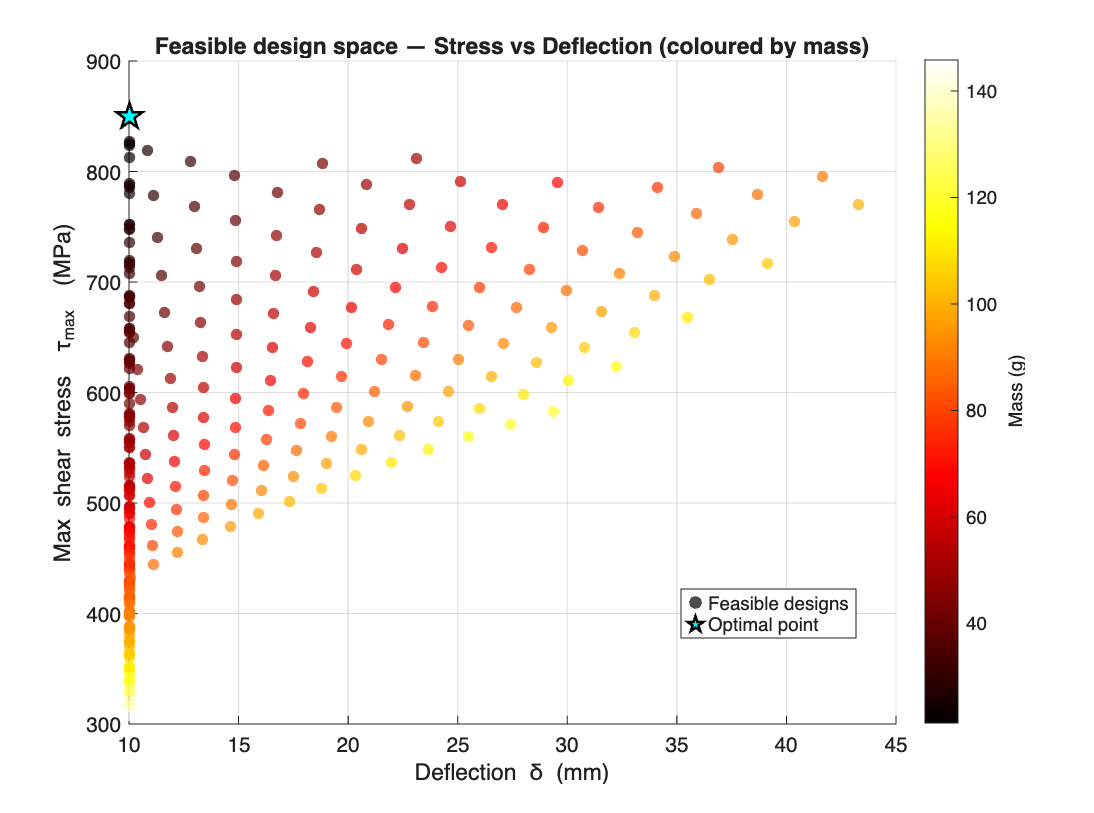
\includegraphics[width=\columnwidth]{fig2_pareto_stress_deflection.png}
  \caption{Feasible designs projected onto the stress--deflection plane and
    coloured by mass; the cyan star identifies the minimum-mass optimum,
    which trades maximum allowable stress for the smallest required deflection.}
  \label{fig:pareto}
\end{figure}

\subsection{Sensitivity Analysis}

Figure~\ref{fig:sens} shows how the optimal mass responds to $\pm10\%$
tightening or relaxation of each constraint.
The allowable stress (Constraint~1) dominates: a \SI{10}{\percent} increase
in $\tau_{\text{allow}}$ yields approximately \SI{18}{\percent} reduction in
mass, making it the highest-leverage lever for mass reduction.
The minimum deflection (Constraint~5) shows moderate sensitivity, while the
surge-frequency ratio, buckling limit, and spring-index bounds have negligible
influence on mass at the current operating point.

\begin{figure}[H]
  \centering
  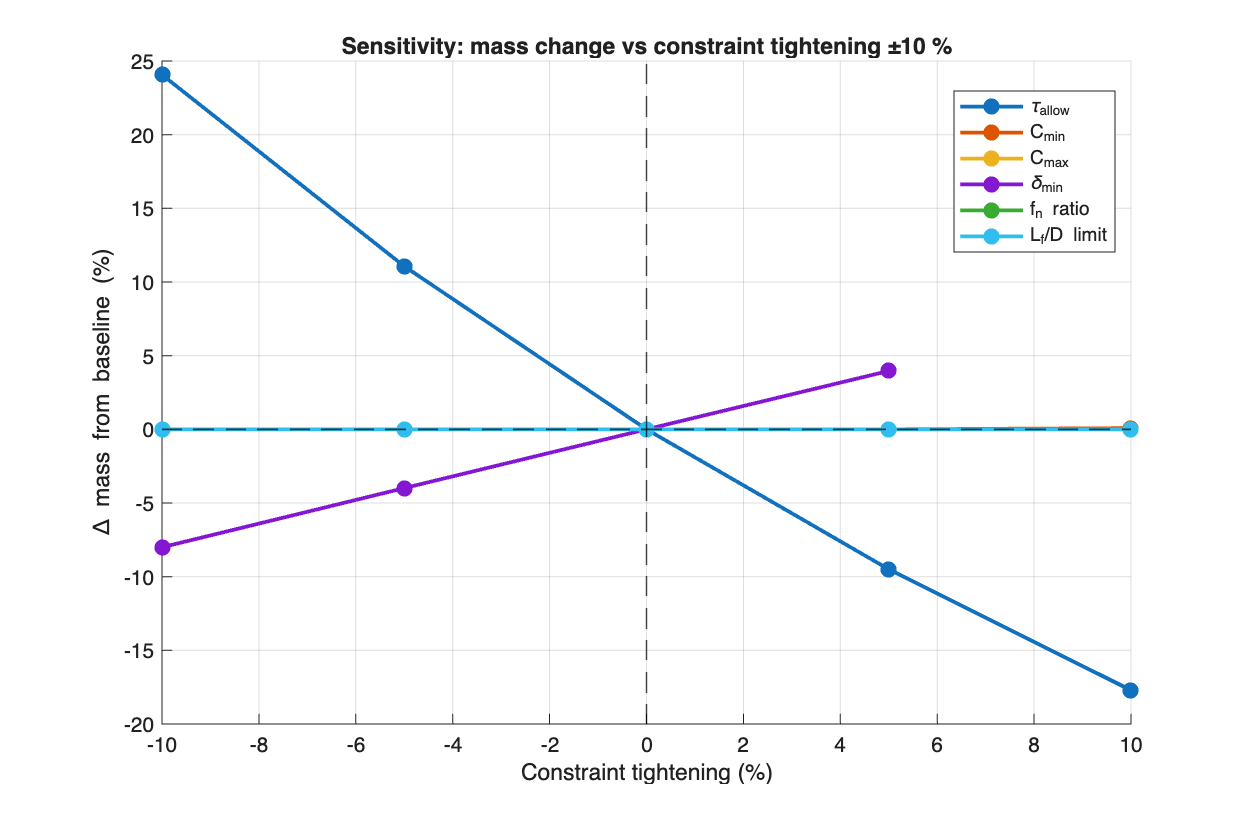
\includegraphics[width=\columnwidth]{fig3_sensitivity.png}
  \caption{Percentage change in optimal spring mass as each constraint is
    independently tightened (positive $x$) or relaxed (negative $x$) by up
    to \SI{10}{\percent}; the allowable stress is the dominant driver.}
  \label{fig:sens}
\end{figure}

\subsection{Spring Rate Surface}

Figure~\ref{fig:ksurf} illustrates how spring rate varies across the $(D,\,d)$
plane at the optimal coil count $N_a = 7.77$.
The strong dependence on $D$ (rate scales as $D^{-3}$) is evident from the
steep gradient along the $D$-axis.

\begin{figure}[H]
  \centering
  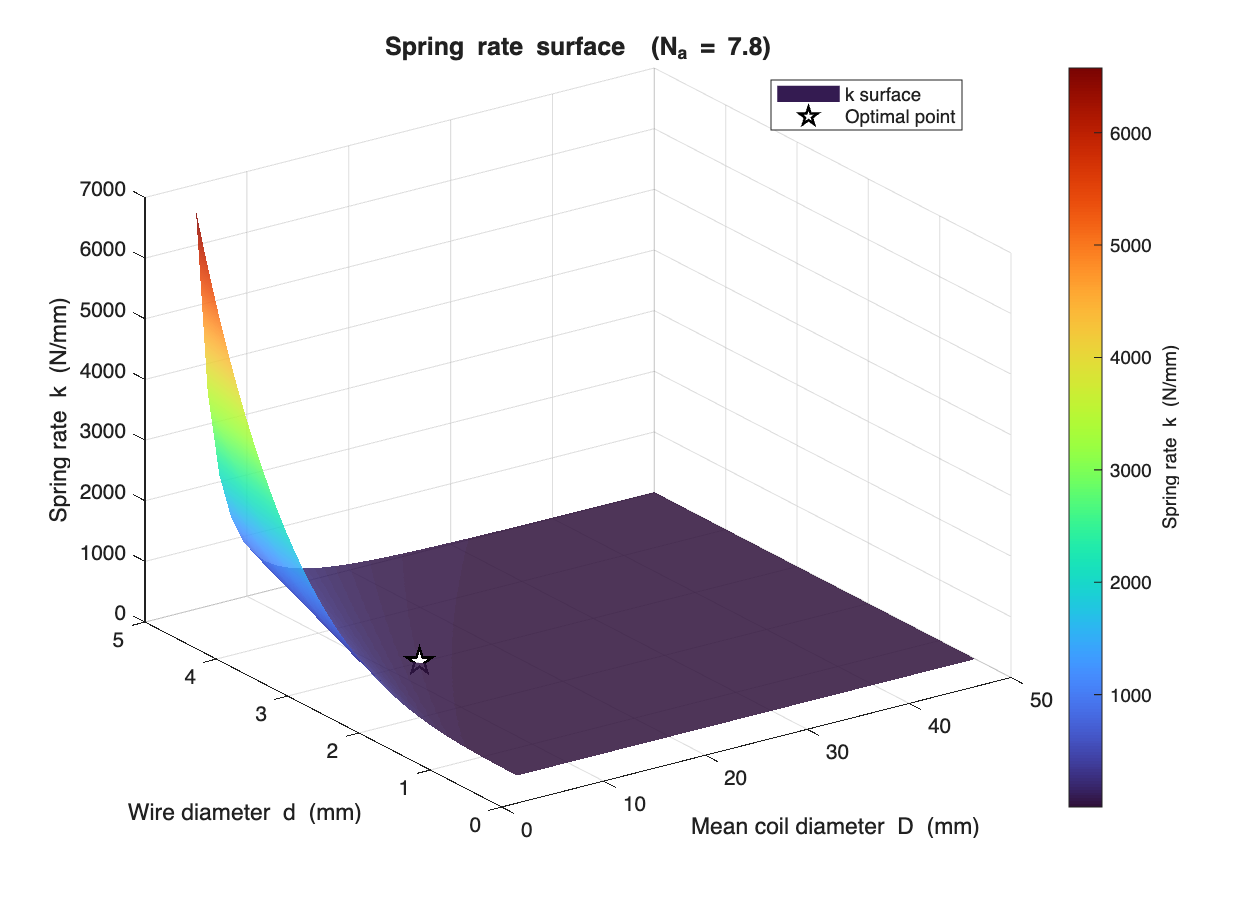
\includegraphics[width=\columnwidth]{fig4_spring_rate_surface.png}
  \caption{Spring rate $k$ (\si{N/mm}) surface as a function of coil geometry
    at $N_a = 7.77$; the cubic inverse dependence on $D$ causes a sharp
    stiffening as coil diameter decreases toward the $C=4$ boundary.}
  \label{fig:ksurf}
\end{figure}

% ==========================================================================
\section{Discussion}
% ==========================================================================

\subsection{Binding Constraints and Optimiser Behaviour}

The simultaneous activation of the stress limit and the $C_{\min}$ bound is
physically intuitive.
Reducing coil diameter $D$ decreases wire length (hence mass) directly and
also reduces the bending-moment arm in the shear-stress formula, Eq.~\eqref{eq:tau}.
The optimiser therefore drives $D$ downward until the spring index reaches the
minimum allowable value $C = 4$; at that point, any further reduction in $D$
would require a proportional reduction in $d$, which simultaneously drives
$\tau_{\text{allow}}$ down (through the $S_{ut}(d)$ dependence) while
$\tau_{\max}$ rises.
The optimum is the saddle point of these two competing effects.

\subsection{Implications of Unity Safety Factor}

A stress safety factor of $\text{SF} = 1.00$ is a theoretical minimum that
is not appropriate for production hardware.
A more conservative target of $\text{SF} = 1.5$ would require $\tau_{\max}$
to be reduced to $\tfrac{2}{3}\,\tau_{\text{allow}}$, necessitating a larger
wire diameter and hence greater mass.
Based on the sensitivity gradient in Fig.~\ref{fig:sens}, imposing $\text{SF}
= 1.5$ (equivalent to tightening the effective stress limit by $\sim\!33\%$)
would increase optimal mass by roughly \SI{50}{g} to approximately \SI{71}{g}
--- a \SI{236}{\percent} increase relative to the theoretical minimum.
This underscores that the stress constraint is the most weight-critical
design driver.

\subsection{Surge Margin and Potential Mass Recovery}

The surge safety factor $f_n / f_{\text{op}} = 86$ greatly exceeds the
required 13.
If the application permits relaxing this ratio to, for example, 20
(still conservative), the surge constraint would no longer influence the
feasible space, and no mass recovery would result at this operating point
because surge is already non-binding.
However, for higher operating frequencies (e.g., $f_{\text{op}} = \SI{100}{Hz}$
in a high-speed cam mechanism), surge avoidance becomes a binding constraint
and directly limits the maximum allowable $N_a$, which in turn forces a stiffer,
heavier spring.

\subsection{Static vs.\ Fatigue Loading}

The Zimmerli criterion $\tau_{\text{allow}} = 0.45\,S_{ut}$ is appropriate
for static or infrequently cycled springs.
For springs subjected to repeated loading (valve springs, clutch springs),
the Goodman endurance diagram must replace the static criterion.
The corrected endurance limit for music wire is typically
$S_{se} \approx 0.45\,S_{ut} / 1.5 \approx 0.30\,S_{ut}$ for infinite life,
which would lower $\tau_{\text{allow}}$ substantially and increase the
minimum-mass design accordingly.

% ==========================================================================
\section{Conclusion}
% ==========================================================================

This study determined the minimum-mass helical compression spring from
ASTM A228 music wire under a complete set of engineering constraints.
The key findings are:

\begin{enumerate}[leftmargin=*,label=\arabic*.]
  \item The optimal design ($d = \SI{2.965}{mm}$, $D = \SI{12.665}{mm}$,
    $N_a = 7.77$, $m = \SI{21.1}{g}$) sits at the intersection of the
    stress boundary and the $C = 4$ manufacturability line.
  \item The \texttt{fmincon} interior-point solver and the independent
    $40\times40$ parametric sweep converge to the same design, validating
    the global optimality of the result.
  \item The dominant design driver is allowable shear stress: a
    \SI{10}{\percent} relaxation of the Zimmerli criterion yields an
    \SI{18}{\percent} mass reduction.
  \item The surge margin (\SI{86}{\times}) is conservatively large at this
    operating frequency; for higher-speed applications, surge avoidance
    would become a binding and mass-critical constraint.
\end{enumerate}

Recommended next steps include: (i)~fatigue life analysis using the
Goodman diagram for cyclic loading, (ii)~assessment of end-condition effects
on effective coil count, (iii)~finite element validation of the
Wahl-corrected stress prediction, and (iv)~manufacturing feasibility review
for the $C = 4$ coil-to-wire ratio with the selected wire diameter.

% ── References ────────────────────────────────────────────────────────────
\begin{thebibliography}{9}

\bibitem{wahl1963}
A.~M.~Wahl,
\textit{Mechanical Springs}, 2nd~ed.
McGraw-Hill, New York, 1963.

\bibitem{shigley2014}
R.~G.~Budynas and J.~K.~Nisbett,
\textit{Shigley's Mechanical Engineering Design}, 10th~ed.
McGraw-Hill, New York, 2014.

\bibitem{byrd1999}
R.~H.~Byrd, M.~E.~Hribar, and J.~Nocedal,
``An interior point algorithm for large-scale nonlinear programming,''
\textit{SIAM J.\ Optim.}, vol.~9, no.~4, pp.~877--900, 1999.

\bibitem{astm_a228}
ASTM~A228/A228M-22,
\textit{Standard Specification for Steel Wire, Music Spring Quality}.
ASTM International, West Conshohocken, PA, 2022.

\bibitem{assoc_spring}
Associated Spring,
\textit{Engineering Guide to Spring Design}.
Barnes Group Inc., Bristol, CT, 1987.

\end{thebibliography}

\end{document}